\documentclass[dvipdfmx,a4paper,uplatex]{jsarticle}
%\usepackage{tetsuryoku}
\usepackage{emath}
\usepackage{tikz}
%\usepgflibrary{arrows.meta}
\usetikzlibrary{arrows.meta}

\usetikzlibrary{angles,calc,intersections, through}
\begin{document}

\begin{center}




%%%%%%%%%%%%%%%%%%%%%%%%%%%%%%%%%%%%%%%%%%%%%%%%%%%%%%% 

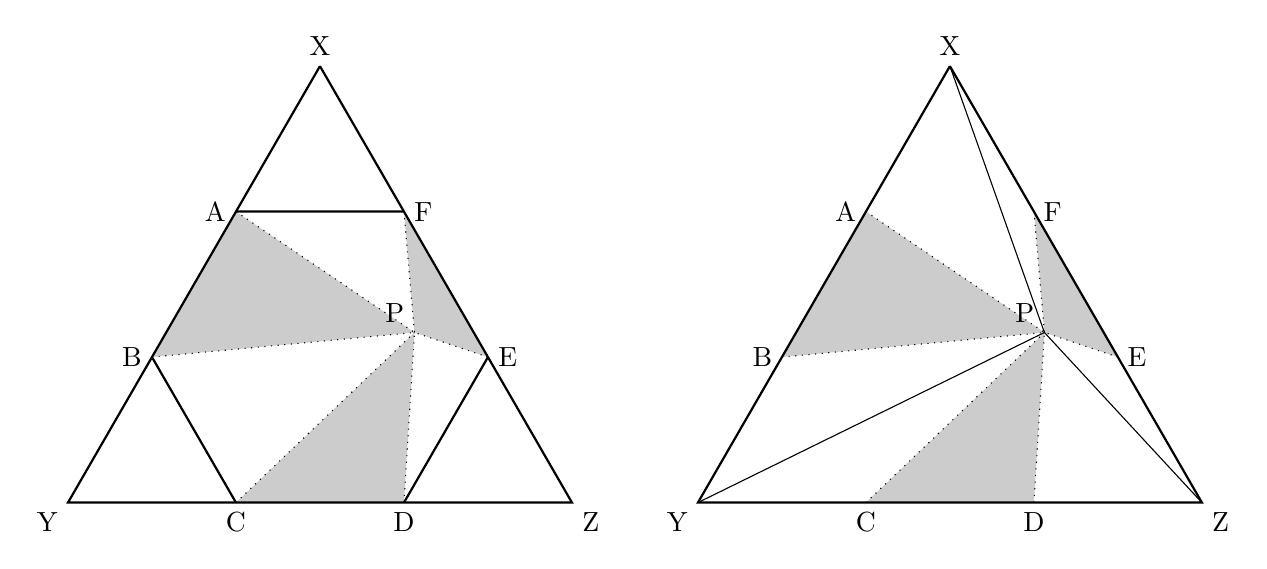
\begin{tikzpicture}[domain=-2.6:2.6,samples=70,scale=0.8]
    \usetikzlibrary{angles,calc}
		
		\coordinate (X) at (0,{sqrt(48)});
		\coordinate (Y) at (-4,0) ; 
		\coordinate (Z) at (4,0);
		
		\draw [thick] (X) node [above] {X} -- (Y) node [below left] {Y} -- (Z) node [below right] {Z}  -- (X);


		\coordinate (A) at ($ (X)!{1/3}!(Y) $);
		\coordinate (B) at ($ (X)!{2/3}!(Y) $);
		\coordinate (C) at ($ (Y)!{1/3}!(Z) $);
		\coordinate (D) at ($ (Y)!{2/3}!(Z) $);
		\coordinate (E) at ($ (Z)!{1/3}!(X) $);
		\coordinate (F) at ($ (Z)!{2/3}!(X) $);
		
		\coordinate (P) at (1.5, 2.7);
		
		
		\draw [thick] (A) node [left] {A} -- (F) node [right] {F};
		\draw [thick] (B) node [left] {B} -- (C) node [below] {C};
		\draw [thick] (D) node [below] {D} -- (E) node [right] {E};
		
		\foreach \y in {A,B,...,F}
			\draw [dotted] (\y) -- (P) ;
			
		\fill [black!, opacity=0.2] (A)--(B)--(P);
		\fill [black!, opacity=0.2] (C)--(D)--(P);
		\fill [black!, opacity=0.2] (E)--(F)--(P);
		
		\draw [thick] (P) node [above left] {P};
		
		
		
		
		
		\coordinate (X) at (10,{sqrt(48)});
		\coordinate (Y) at (6,0) ; 
		\coordinate (Z) at (14,0);
		
		\draw [thick] (X) node [above] {X} -- (Y) node [below left] {Y} -- (Z) node [below right] {Z}  -- (X);


		\coordinate (A) at ($ (X)!{1/3}!(Y) $);
		\coordinate (B) at ($ (X)!{2/3}!(Y) $);
		\coordinate (C) at ($ (Y)!{1/3}!(Z) $);
		\coordinate (D) at ($ (Y)!{2/3}!(Z) $);
		\coordinate (E) at ($ (Z)!{1/3}!(X) $);
		\coordinate (F) at ($ (Z)!{2/3}!(X) $);
		
		\coordinate (P) at (11.5, 2.7);
		
		\draw  (A) node [left] {A};
		\draw  (B) node [left] {B};
		\draw  (C) node [below] {C};
		\draw  (D) node [below] {D};
		\draw  (E) node [right] {E};
		\draw  (F) node [right] {F};
		
		\foreach \y in {A,B,...,F}
			\draw [dotted](\y) -- (P) ;
		\foreach \y in {X,Y,Z}
			\draw [] (\y) -- (P) ;
			
		\fill [black!, opacity=0.2] (A)--(B)--(P);
		\fill [black!, opacity=0.2] (C)--(D)--(P);
		\fill [black!, opacity=0.2] (E)--(F)--(P);
		
		\draw [thick] (P) node [above left] {P};
\end{tikzpicture}


\bigskip

\newpage
%%%%%%%%%%%%%%%%%%%%%%%%%%%%%%%%%%%%%%%%%%%%%%%%%%%%%%% 

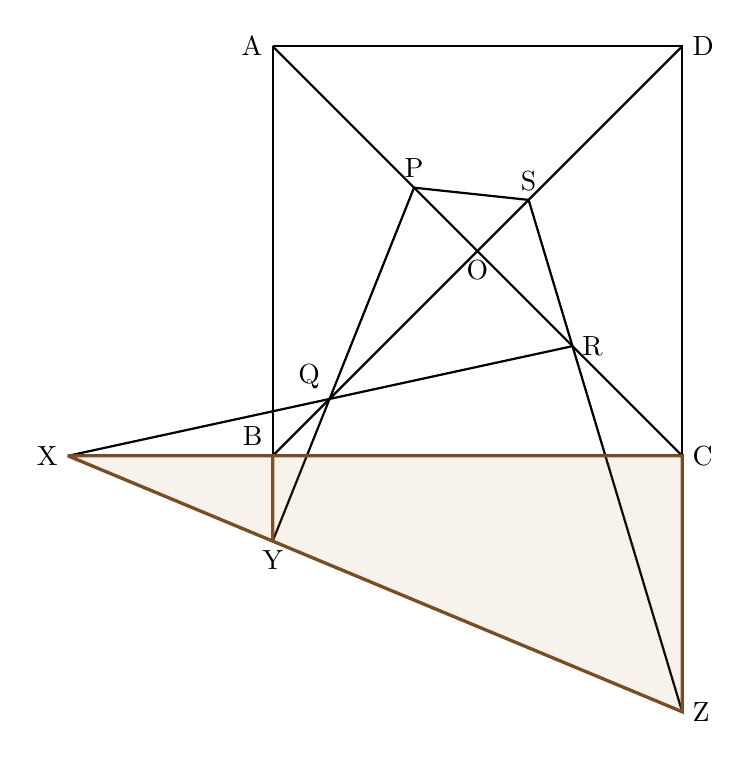
\begin{tikzpicture}[domain=-2.6:2.6,samples=70,scale=0.65]
    \usetikzlibrary{angles,calc,intersections}
		
		\coordinate (O) at (0,0);
		\coordinate (A) at (-4,4) ; 
		\coordinate (B) at (-4,-4);
		\coordinate (C) at (4,-4);
		\coordinate (D) at (4,4);
		\coordinate (S) at (1,1);
		
		
		\draw [thick] (A) node [left] {A} -- (B) node [above left] {B} -- (C) node [right] {C} -- (D) node [right] {D} --(A);
		
		\draw (S) node [above] {S};
		\draw (O) node [below] {O};
		
		\foreach \y in {A,B,C,D}
			\draw [thick] (\y) -- (O) ;
			
			
		\coordinate (X) at (-8,-4);%%%%%%%%%%%%%%%%%%
		\draw [thick] (X) node [left] {X};
		\coordinate (Z) at (4,-9);%%%%%%%%%%%%%%%%%%%%%%%このX,Zの位置で残りは自動で定まる
		\draw [thick] (Z) node [right] {Z};
		%\coordinate (X) at (-8,-4);
		
		\path [name path = CD] (4,-8)--(D);
		\path [name path = AB] (-4,-8)--(A);
		\path [name path = BD] (B)--(D);
		\path [name path = AC] (A)--(C);
		\draw[name path = XZ, thick] (X) -- (Z);
		\path [name intersections={of=AB and XZ,by={[label=below:Y]Y}}];
		
		
		
		%\path [name path = ab, draw, thick] (A)--(-4,-16/3) node [below] {Y};
		

		\draw[thick] (X) -- (B)--(Y);
		\draw[thick] (C) -- (Z);
		
		\draw[name path = SZ, thick] (S) -- (Z);
		
		\path [name intersections={of=SZ and AC,by={[label=right:R]R}}];
		
		\draw[name path = XR, thick] (X) -- (R);
		
		\path [name intersections={of=XR and BD,by={[label=above left:Q]Q}}];
		
		
		\coordinate (W) at ($ (Y)!3!(Q) $);
		\path [name path = YQ] (Y)--(W);
		
		\path [name intersections={of=YQ and AC,by={[label=above :P]P}}];
		
		\draw [thick] (Y)--(Q)--(P)--(S);
		
		\draw [very thick, brown!60!black] (X)--(C)--(Z)--(X);
		\draw [very thick, brown!60!black] (B)--(Y);
		\fill [brown,opacity=0.1] (X)--(C)--(Z)--(X);
		
		
\end{tikzpicture}%
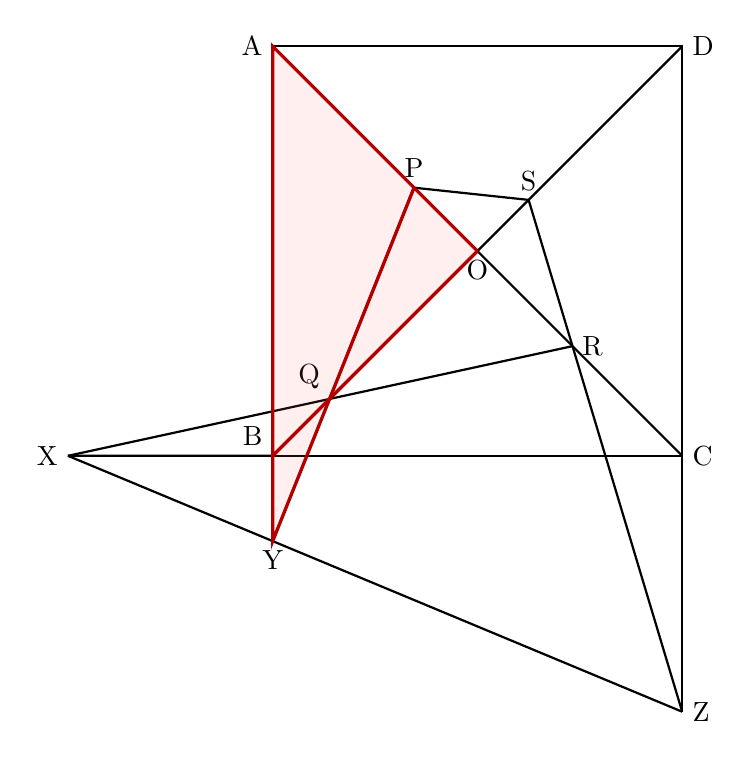
\begin{tikzpicture}[domain=-2.6:2.6,samples=70,scale=0.65]
    \usetikzlibrary{angles,calc,intersections}
		
		\coordinate (O) at (0,0);
		\coordinate (A) at (-4,4) ; 
		\coordinate (B) at (-4,-4);
		\coordinate (C) at (4,-4);
		\coordinate (D) at (4,4);
		\coordinate (S) at (1,1);
		
		
		\draw [thick] (A) node [left] {A} -- (B) node [above left] {B} -- (C) node [right] {C} -- (D) node [right] {D} --(A);
		
		\draw (S) node [above] {S};
		\draw (O) node [below] {O};
		
		\foreach \y in {A,B,C,D}
			\draw [thick] (\y) -- (O) ;
			
			
		\coordinate (X) at (-8,-4);%%%%%%%%%%%%%%%%%%
		\draw [thick] (X) node [left] {X};
		\coordinate (Z) at (4,-9);%%%%%%%%%%%%%%%%%%%%%%%このX,Zの位置で残りは自動で定まる
		\draw [thick] (Z) node [right] {Z};
		%\coordinate (X) at (-8,-4);
		
		\path [name path = CD] (4,-8)--(D);
		\path [name path = AB] (-4,-8)--(A);
		\path [name path = BD] (B)--(D);
		\path [name path = AC] (A)--(C);
		\draw[name path = XZ, thick] (X) -- (Z);
		\path [name intersections={of=AB and XZ,by={[label=below:Y]Y}}];
		
		
		
		%\path [name path = ab, draw, thick] (A)--(-4,-16/3) node [below] {Y};
		

		\draw[thick] (X) -- (B)--(Y);
		\draw[thick] (C) -- (Z);
		
		\draw[name path = SZ, thick] (S) -- (Z);
		
		\path [name intersections={of=SZ and AC,by={[label=right:R]R}}];
		
		\draw[name path = XR, thick] (X) -- (R);
		
		\path [name intersections={of=XR and BD,by={[label=above left:Q]Q}}];
		
		
		\coordinate (W) at ($ (Y)!3!(Q) $);
		\path [name path = YQ] (Y)--(W);
		
		\path [name intersections={of=YQ and AC,by={[label=above :P]P}}];
		
		\draw [thick] (Y)--(Q)--(P)--(S);
		
		\fill [red!60, opacity=0.1] (O)--(A)--(Y)--(Q)--(O);
		
		\draw [very thick,red!70!black] (O)--(A)--(B)--(O);
		\draw [very thick,red!70!black] (P)--(Q)--(Y)--(B);
		
\end{tikzpicture}

\bigskip

\bigskip



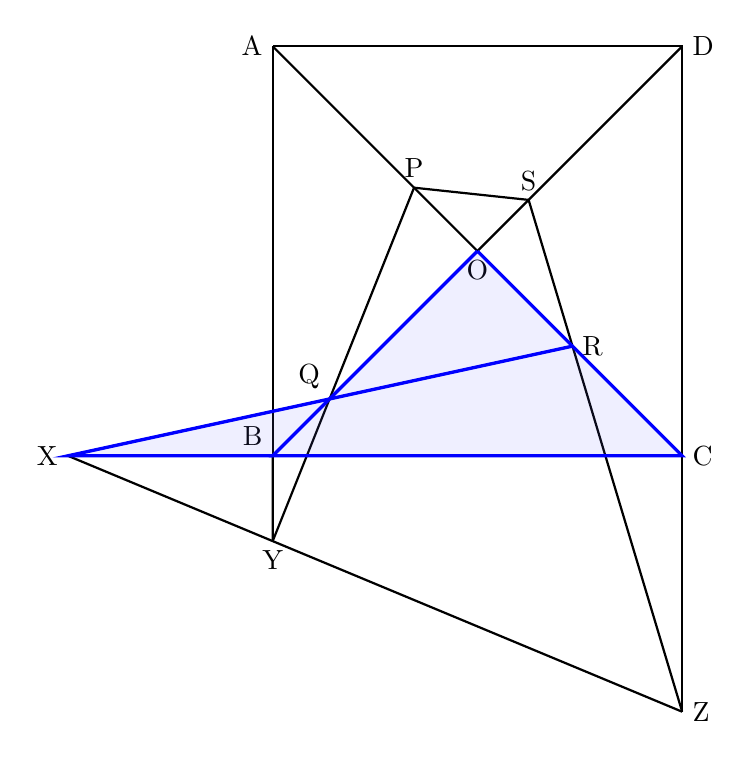
\begin{tikzpicture}[domain=-2.6:2.6,samples=70,scale=0.65]
    \usetikzlibrary{angles,calc,intersections}
		
		\coordinate (O) at (0,0);
		\coordinate (A) at (-4,4) ; 
		\coordinate (B) at (-4,-4);
		\coordinate (C) at (4,-4);
		\coordinate (D) at (4,4);
		\coordinate (S) at (1,1);
		
		
		\draw [thick] (A) node [left] {A} -- (B) node [above left] {B} -- (C) node [right] {C} -- (D) node [right] {D} --(A);
		
		\draw (S) node [above] {S};
		\draw (O) node [below] {O};
		
		\foreach \y in {A,B,C,D}
			\draw [thick] (\y) -- (O) ;
			
			
		\coordinate (X) at (-8,-4);%%%%%%%%%%%%%%%%%%
		\draw [thick] (X) node [left] {X};
		\coordinate (Z) at (4,-9);%%%%%%%%%%%%%%%%%%%%%%%このX,Zの位置で残りは自動で定まる
		\draw [thick] (Z) node [right] {Z};
		%\coordinate (X) at (-8,-4);
		
		\path [name path = CD] (4,-8)--(D);
		\path [name path = AB] (-4,-8)--(A);
		\path [name path = BD] (B)--(D);
		\path [name path = AC] (A)--(C);
		\draw[name path = XZ, thick] (X) -- (Z);
		\path [name intersections={of=AB and XZ,by={[label=below:Y]Y}}];
		
		
		
		%\path [name path = ab, draw, thick] (A)--(-4,-16/3) node [below] {Y};
		

		\draw[thick] (X) -- (B)--(Y);
		\draw[thick] (C) -- (Z);
		
		\draw[name path = SZ, thick] (S) -- (Z);
		
		\path [name intersections={of=SZ and AC,by={[label=right:R]R}}];
		
		\draw[name path = XR, thick] (X) -- (R);
		
		\path [name intersections={of=XR and BD,by={[label=above left:Q]Q}}];
		
		
		\coordinate (W) at ($ (Y)!3!(Q) $);
		\path [name path = YQ] (Y)--(W);
		
		\path [name intersections={of=YQ and AC,by={[label=above :P]P}}];
		
		\draw [thick] (Y)--(Q)--(P)--(S);
		
		\fill [blue!60, opacity=0.1] (O)--(C)--(X)--(Q)--(O);
		
		\draw [very thick,blue] (O)--(B)--(C)--(O);
		\draw [very thick,blue] (R)--(Q)--(X)--(B);
		
		
\end{tikzpicture}%
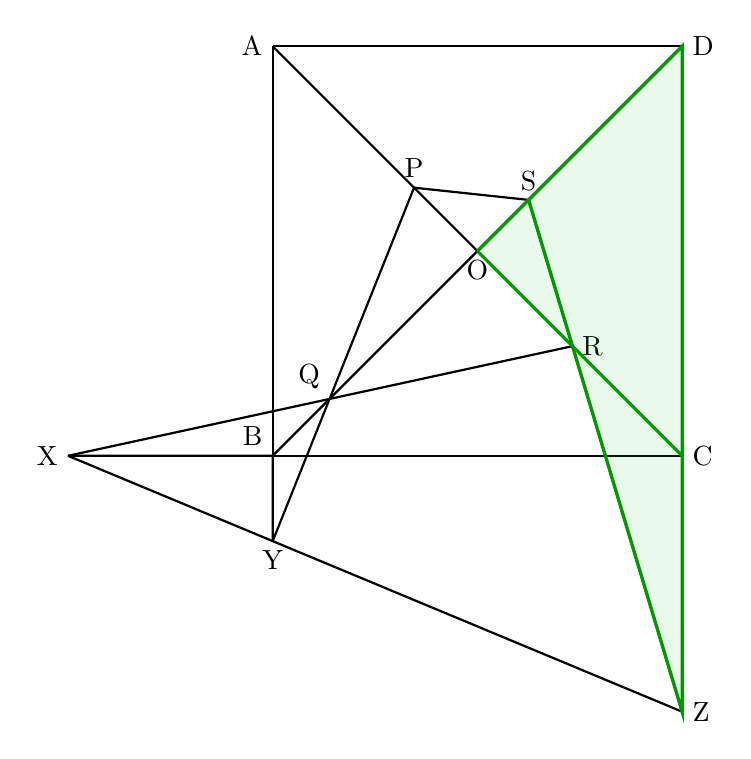
\begin{tikzpicture}[domain=-2.6:2.6,samples=70,scale=0.65]
    \usetikzlibrary{angles,calc,intersections}
		
		\coordinate (O) at (0,0);
		\coordinate (A) at (-4,4) ; 
		\coordinate (B) at (-4,-4);
		\coordinate (C) at (4,-4);
		\coordinate (D) at (4,4);
		\coordinate (S) at (1,1);
		
		
		\draw [thick] (A) node [left] {A} -- (B) node [above left] {B} -- (C) node [right] {C} -- (D) node [right] {D} --(A);
		
		\draw (S) node [above] {S};
		\draw (O) node [below] {O};
		
		\foreach \y in {A,B,C,D}
			\draw [thick] (\y) -- (O) ;
			
			
		\coordinate (X) at (-8,-4);%%%%%%%%%%%%%%%%%%
		\draw [thick] (X) node [left] {X};
		\coordinate (Z) at (4,-9);%%%%%%%%%%%%%%%%%%%%%%%このX,Zの位置で残りは自動で定まる
		\draw [thick] (Z) node [right] {Z};
		%\coordinate (X) at (-8,-4);
		
		\path [name path = CD] (4,-8)--(D);
		\path [name path = AB] (-4,-8)--(A);
		\path [name path = BD] (B)--(D);
		\path [name path = AC] (A)--(C);
		\draw[name path = XZ, thick] (X) -- (Z);
		\path [name intersections={of=AB and XZ,by={[label=below:Y]Y}}];
		
		
		
		%\path [name path = ab, draw, thick] (A)--(-4,-16/3) node [below] {Y};
		

		\draw[thick] (X) -- (B)--(Y);
		\draw[thick] (C) -- (Z);
		
		\draw[name path = SZ, thick] (S) -- (Z);
		
		\path [name intersections={of=SZ and AC,by={[label=right:R]R}}];
		
		\draw[name path = XR, thick] (X) -- (R);
		
		\path [name intersections={of=XR and BD,by={[label=above left:Q]Q}}];
		
		
		\coordinate (W) at ($ (Y)!3!(Q) $);
		\path [name path = YQ] (Y)--(W);
		
		\path [name intersections={of=YQ and AC,by={[label=above :P]P}}];
		
		\draw [thick] (Y)--(Q)--(P)--(S);
		
		\fill [green!60!gray, opacity=0.1] (O)--(D)--(Z)--(R)--(O);
		
		\draw [very thick,green!60!black] (O)--(C)--(D)--(O);
		\draw [very thick,green!60!black] (S)--(R)--(Z)--(C);
		
\end{tikzpicture}





\newpage

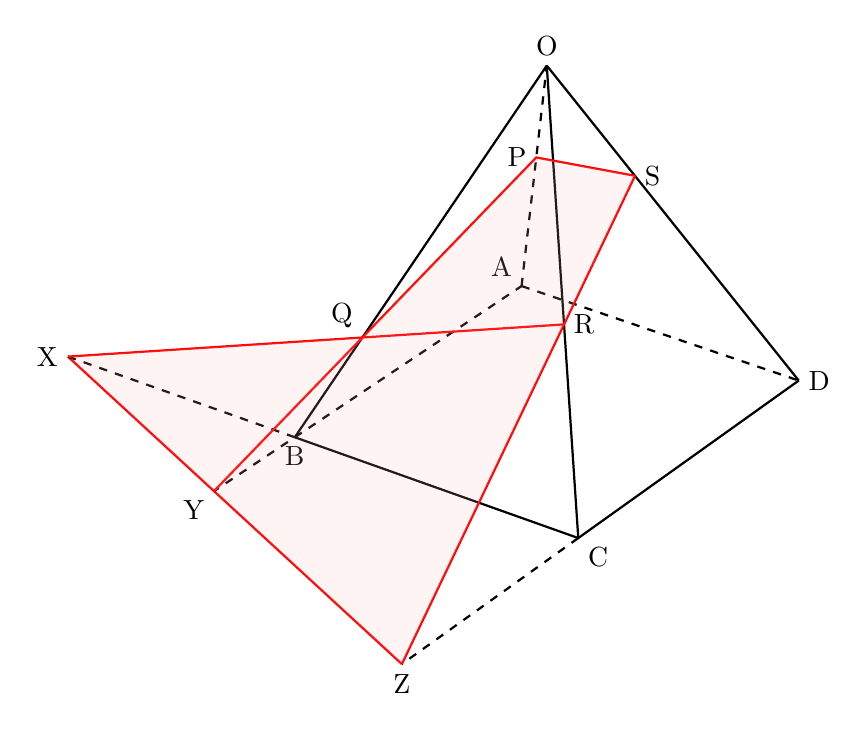
\begin{tikzpicture}[domain=-2.6:2.6,samples=70,scale=0.8]
    \usetikzlibrary{angles,calc,intersections}
		
		\coordinate (O) at (0,5.5);
		\coordinate (A) at (-0.4,2) ; 
		\coordinate (B) at (-4,-0.4);
		\coordinate (C) at (0.5,-2);
		\coordinate (D) at (4,0.5);
		\coordinate (S) at ($ (O)!0.35!(D) $);
		
		
		\draw (A) node [above left] {A};
		\draw (B) node [below] {B};
		\draw (C) node [below right] {C};
		\draw (D) node [right] {D};
		\draw (S) node [right] {S};
		\draw (O) node [above] {O};
		
		\draw [thick] (B)--(C)--(D);
		\draw [thick,dashed] (B)--(A);
		\draw [thick,dashed] (A)--(D);
		
		\foreach \y in {B,C,D}
			\draw [thick] (\y) -- (O) ;
		\draw [thick,dashed] (A) -- (O) ;
		
		\coordinate (X) at ($ (C)!1.8!(B) $);%%%%%%%%%%%%%%%%%%
		\draw [thick] (X) node [left] {X};
		\coordinate (Z) at ($ (D)!1.8!(C) $);%%%%%%%%%%%%%%%%%%%%%%%このX,Zの位置で残りは自動で定まる
		\draw [thick] (Z) node [below] {Z};
		
		\path [name path = CD] (Z)--(D);
		\path [name path = AB] ($ (A)!1.5!(B) $)--(A);
		\path [name path = OD] (O)--(D);
		\path [name path = OC] (O)--(C);
		\path [name path = OB] (O)--(B);
		\path [name path = OA] (O)--(A);
		\draw[name path = XZ, thick, red] (X) -- (Z);
		\path [name intersections={of=AB and XZ,by={[label=below left:Y]Y}}];
		
		\draw[thick, dashed] (X) -- (B) -- (Y);
		\draw[thick, dashed] (C) -- (Z);
		
		\draw[name path = SZ, thick, red] (S) -- (Z);
		
		\path [name intersections={of=SZ and OC,by={[label=right:R]R}}];
		
		\draw[name path = XR, thick, red] (X) -- (R);
		
		\path [name intersections={of=XR and OB,by={[label=above left:Q]Q}}];
		
		
		\coordinate (W) at ($ (Y)!3!(Q) $);
		\path [name path = YQ] (Y)--(W);
		
		\path [name intersections={of=YQ and OA,by={[label=left:P]P}}];
		
		\draw [thick,red] (Y)--(Q)--(P)--(S);
		%\draw [very thick,red] (P)--(Q)--(R)--(S)--(P);
		\fill [red!30, opacity=0.15] (P)--(Q)--(X)--(Z)--(S)--(P);
		
		
\end{tikzpicture}








%%%%%%%%%%%%%%%%%%%%%%%%%%%%%%%%%%%%%%%%%%%
\begin{tikzpicture}[domain=-2.6:2.6,samples=70,scale=1.2]
    \usetikzlibrary{angles}
		
		\coordinate (P) at (0,0) ;
		\coordinate (Q) at (5,3) ; 
		\coordinate (A) at (1,0) ;
		\coordinate (B) at (1,1) ;
		\coordinate (C) at (2,1) ;
		\coordinate (D) at (2,1.8) ;
		\coordinate (E) at (5,1.8) ;
		
		
		\draw[thick] (P) node [below] {P} --(A)--(B)--(C)--(D)--(E)--(Q) node [right] {${\rm Q}$};
		
		%\draw (b)  node [right] {${\rm B}$};
		%\draw (c)  node [above] {${\rm C}$};
		
		
		
		
		\draw [] ($(A)!7pt!(P)$)--($(A)!7pt!(P)!7pt!90:(A)$)--($(A)!7pt!(B)$); %角度
		\draw [] ($(B)!7pt!(A)$)--($(B)!7pt!(A)!7pt!270:(B)$)--($(B)!7pt!(C)$);
		\draw [] ($(C)!7pt!(B)$)--($(C)!7pt!(B)!7pt!90:(C)$)--($(C)!7pt!(D)$);
		\draw [] ($(D)!7pt!(C)$)--($(D)!7pt!(C)!7pt!270:(D)$)--($(D)!7pt!(E)$);
		\draw [] ($(E)!7pt!(D)$)--($(E)!7pt!(D)!7pt!90:(E)$)--($(E)!7pt!(Q)$);
\end{tikzpicture}











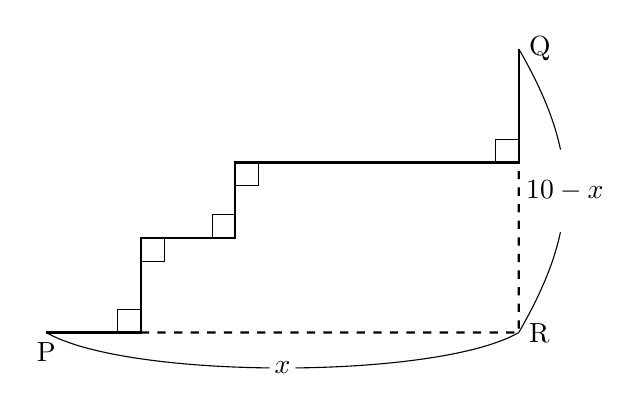
\begin{tikzpicture}[domain=-2.6:2.6,samples=70,scale=1.2]
    \usetikzlibrary{angles}
		
		\coordinate (P) at (0,0) ;
		\coordinate (Q) at (5,3) ; 
		\coordinate (A) at (1,0) ;
		\coordinate (B) at (1,1) ;
		\coordinate (C) at (2,1) ;
		\coordinate (D) at (2,1.8) ;
		\coordinate (E) at (5,1.8) ;
		
		
		\draw[thick] (P) node [below] {P} --(A)--(B)--(C)--(D)--(E)--(Q) node [right] {${\rm Q}$};
		
		\draw[thick, dashed] (A)--(5,0) node [right] {R} --(E);
		\draw [bend right,distance=1cm] (P)
         to node [fill=white,inner sep=0.8pt,circle] {$x$} (5,0); %長さ
         \draw [bend right,distance=1.3cm] (5,0)
         to node [fill=white,inner sep=0.5pt,circle] {$10-x$} (Q); %長さ

		%\draw (b)  node [right] {${\rm B}$};
		%\draw (c)  node [above] {${\rm C}$};
		
		
		
		
		\draw [] ($(A)!7pt!(P)$)--($(A)!7pt!(P)!7pt!90:(A)$)--($(A)!7pt!(B)$); %角度
		\draw [] ($(B)!7pt!(A)$)--($(B)!7pt!(A)!7pt!270:(B)$)--($(B)!7pt!(C)$);
		\draw [] ($(C)!7pt!(B)$)--($(C)!7pt!(B)!7pt!90:(C)$)--($(C)!7pt!(D)$);
		\draw [] ($(D)!7pt!(C)$)--($(D)!7pt!(C)!7pt!270:(D)$)--($(D)!7pt!(E)$);
		\draw [] ($(E)!7pt!(D)$)--($(E)!7pt!(D)!7pt!90:(E)$)--($(E)!7pt!(Q)$);
\end{tikzpicture}




\begin{tikzpicture}[domain=-2.6:2.6,samples=70,scale=1.2]
    \usetikzlibrary{angles}
		
		\coordinate (A) at (0,0) node [left] {${\rm A}$};
		\coordinate (B) at (3,0) ; 
		\coordinate (C) at (0,4) ;
		\coordinate (P) at (0.5,1.2) ;
		
		
		\draw (B)  node [right] {${\rm B}$};
		\draw (C)  node [above] {${\rm C}$};
		\draw (P)  node [left] {${\rm P}$};
		
		\draw [-] (A)--(B)--(C)--(A);
		\foreach \y in {A,B,C}
			\draw [] (\y) -- (P) ;
		
		\draw (0.35,0.48)  node  {$x$};
		\draw (1.62,0.47)  node  {$y$};
		\draw (0.46,2.5)  node  {$z$};
		
		
		
		\draw [] ($(P)!8pt!(A)$)--($(P)!8pt!(A)!8pt!270:(P)$)--($(P)!8pt!(B)$); %角度
		\draw pic [draw, angle radius=4mm,angle eccentricity=1,pic text=$\hspace{2.4zw} 120^{\circ}$] {angle = B--P--C}; %角度
		
\end{tikzpicture}


\begin{tikzpicture}[domain=-2.6:2.6,samples=70,scale=1.2]

		\draw [->,semithick] (-4,0)--(4,0) node [right] {$x$} ;
		\draw [->] (0,-4)--(0,4) node [above] {$y$};
		\coordinate (P) at (1,2) ;
		\coordinate (Q) at (3,1) ; 
		\coordinate (R) at (-3,0.6) ;
		\coordinate (S) at (-0.5,-2.5) ;
		\coordinate (O) at (0,0);
		
		\draw (P) node [above] {P$(a,b)$} ;
		\draw (Q) node [right] {Q$(c,d)$} ;
		\draw (R) node [above] {R$(e,f)$} ;
		\draw (S) node [below] {S$(g,h)$} ;
		\draw (O) node [below left] {O};
		
		\foreach \y in {P,Q,R,S}
			\draw [-{Latex[length=2mm]},very thick] (O) -- (\y) ;
		
		
		
		
\end{tikzpicture}



\newpage


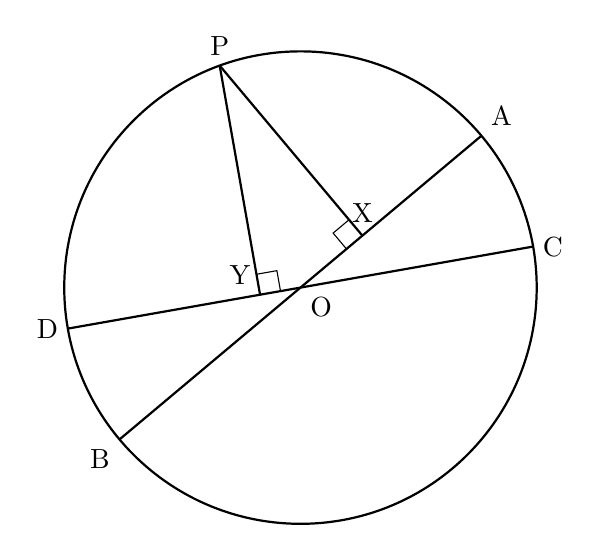
\begin{tikzpicture}[domain=-2.6:2.6,samples=70,scale=1.5]

		\coordinate (A) at (40:2) ;
		\coordinate (B) at (220:2) ; 
		\coordinate (C) at (10:2) ;
		\coordinate (D) at (190:2) ;
		\coordinate (P) at (110:2) ;
		\coordinate (O) at (0,0);
		
		\draw [name path = Circle, thick] (0,0) circle (2);
		
		\draw (A) node [above right] {A} ;
		\draw (B) node [below left] {B} ;
		\draw (C) node [right] {C} ;
		\draw (D) node [left] {D} ;
		\draw (P) node [above] {P} ;
		\draw (O) node [below right] {O};
		
		\draw[name path = AB, thick] (A) -- (B);
		\draw[name path = CD, thick] (C) -- (D);
		
		\coordinate (X) at ($(A)!(P)!(B)$);
		\coordinate (Y) at ($(C)!(P)!(D)$);
		\draw (X) node [above=1.3pt ] {X};
		\draw (Y) node [above left] {Y};
		\draw [thick] (X)--(P);
		\draw [thick] (Y)--(P);
		
		\draw [] ($(X)!5pt!(B)$)--($(X)!5pt!(B)!5pt!90:(X)$)--($(X)!5pt!(P)$);
		\draw [] ($(Y)!5pt!(C)$)--($(Y)!5pt!(C)!5pt!270:(Y)$)--($(Y)!5pt!(P)$);
		
\end{tikzpicture}

\bigskip

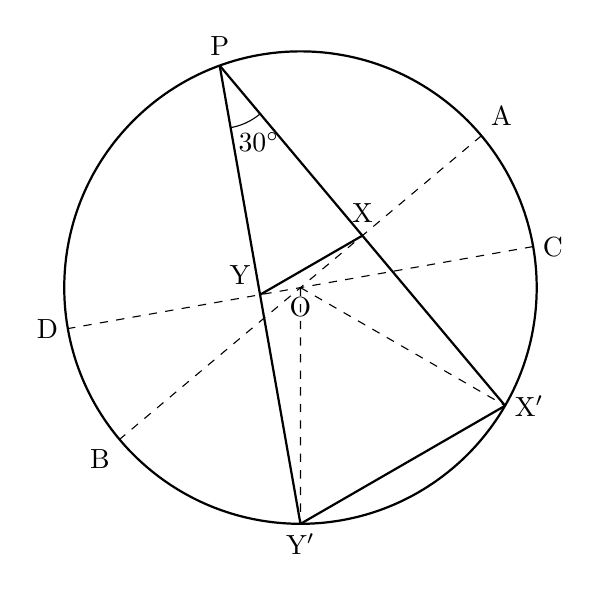
\begin{tikzpicture}[domain=-2.6:2.6,samples=70,scale=1.5]

		\coordinate (A) at (40:2) ;
		\coordinate (B) at (220:2) ; 
		\coordinate (C) at (10:2) ;
		\coordinate (D) at (190:2) ;
		\coordinate (P) at (110:2) ;
		\coordinate (O) at (0,0);
		
		\draw [name path = Circle, thick] (0,0) circle (2);
		
		\draw (A) node [above right] {A} ;
		\draw (B) node [below left] {B} ;
		\draw (C) node [right] {C} ;
		\draw (D) node [left] {D} ;
		\draw (P) node [above] {P} ;
		\draw (O) node [below] {O};
		
		\draw[name path = AB,  dashed] (A) -- (B);
		\draw[name path = CD,  dashed] (C) -- (D);
		
		\coordinate (X) at ($(A)!(P)!(B)$);
		\coordinate (Y) at ($(C)!(P)!(D)$);
		\draw (X) node [above=1.3pt ] {X};
		\draw (Y) node [above left] {Y};
		\draw [thick] (X)--(P);
		\draw [thick] (Y)--(P);
		
		\coordinate (X') at ($ (P)!2!(X) $);
		\draw (X') node [right] {X$'$} ;
		\coordinate (Y') at ($ (P)!2!(Y) $);
		\draw (Y') node [below] {Y$'$} ;
		
		\draw [thick] (X)--(X');
		\draw [thick] (Y)--(Y');
		\draw [thick] (X')--(Y');
		\draw [thick] (X)--(Y);
		\draw [dashed] (O)--(X');
		\draw [dashed] (O)--(Y');
		
		\draw pic [draw, angle radius=8mm,angle eccentricity=1,pic text={}] {angle = Y--P--X}; %角度
		
		\draw [thick] (P)  ++(-63:7.3mm) node [] {$30^{\circ}$};
		
		
		%\draw [] ($(X)!5pt!(B)$)--($(X)!5pt!(B)!5pt!90:(X)$)--($(X)!5pt!(P)$);
		%\draw [] ($(Y)!5pt!(C)$)--($(Y)!5pt!(C)!5pt!270:(Y)$)--($(Y)!5pt!(P)$);
		
\end{tikzpicture}




\newpage


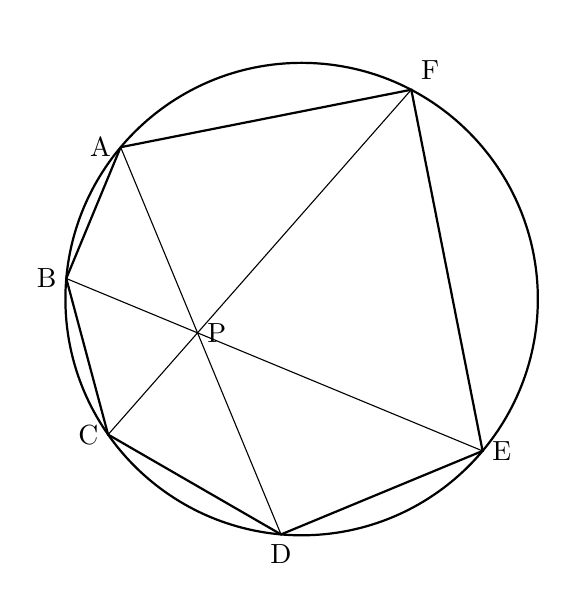
\begin{tikzpicture}[domain=-2.6:2.6,samples=70,scale=1.5]

		\coordinate (A) at (140:2) ;
		\coordinate (B) at (175:2) ; 
		\coordinate (C) at (215:2) ;
		\coordinate (D) at (265:2) ;
		\coordinate (E) at (320:2) ;
		\coordinate (O) at (0,0);
		
		\draw [name path = Circle, thick] (0,0) circle (2);
		
		\draw (A) node [left] {A} ;
		\draw (B) node [left] {B} ;
		\draw (C) node [left] {C} ;
		\draw (D) node [below] {D} ;
		\draw (E) node [right] {E} ;

		
		\draw[name path = AD] (A) -- (D);
		\draw[name path = BE] (B) -- (E);
		
		\path [name intersections={of=AD and BE,by={[label=right:P]P}}];
		
		\coordinate (G) at ($(C)!4!(P)$);
		
		%\draw[name path = CG,  dashed] (C) -- (G);
		\path [name path = CG] (P)--(G);
		\path [name intersections={of=Circle and CG,by={[label=above right:F]F}}];
		
		\draw[name path = CF] (C) -- (F);
		
		\draw [thick] (A)--(B)--(C)--(D)--(E)--(F)--(A);

\end{tikzpicture}



\newpage

\begin{tikzpicture}[domain=-2.6:2.6,samples=70,scale=1]

		\coordinate (A) at (0:5) ;
		\coordinate (B) at (90:5) ; 
		\coordinate (P) at (26:5) ;
		\coordinate (Q) at (64:5) ; 
		\coordinate (X) at ($(0,0)!0.3!(B)$) ;
		
		\draw (A) node [right] {A} ;
		\draw (B) node [left] {B} ;
		\draw (0,0) node [left] {O};
		\draw (P) node [right] {P} ;
		\draw (Q) node [above] {Q} ;
		\draw (X) node [left] {X} ;
		
		\draw (A) [thick] arc [start angle = 0, end angle = 90, radius = 5];
		\draw [thick] (A)--(O)--(B);
		
		\draw [thick] (P)--(X)--(Q);

		
		\draw [bend right,distance=0.9cm] (O)
         to node [fill=white,inner sep=0.8pt,circle] {6} (A); %長さ
\end{tikzpicture}


\begin{tikzpicture}[domain=-2.6:2.6,samples=70,scale=1]

		\coordinate (A) at (0:5) ;
		\coordinate (B) at (90:5) ; 
		\coordinate (P) at (26:5) ;
		\coordinate (Q) at (64:5) ; 
		\coordinate (C) at (180:5) ;
		\coordinate (Q') at (116:5) ;
		\coordinate (X) at ($(0,0)!0.3!(B)$) ;
		
		\draw (A) node [right] {A} ;
		\draw (B) node [above] {B} ;
		\draw (0,0) node [below] {O};
		\draw (P) node [right] {P} ;
		\draw (Q) node [above] {Q} ;
		\draw (Q') node [above] {Q$'$} ;
		\draw (X) node [left] {X} ;
		
		\draw (A) [thick] arc [start angle = 0, end angle = 90, radius = 5];
		\draw (B) [thick, dotted] arc [start angle = 90, end angle = 180, radius = 5];
		\draw [thick] (A)--(O)--(B);
		\draw [thick, dotted] (C)--(O);
		\draw [thick, dotted] (X)--(Q);
		\draw [thick] (P)--(X)--(Q');

		\draw [thick, dashed] (Q')--(O)--(P);
		
		\draw [bend right,distance=0.9cm] (O)
         to node [fill=white,inner sep=0.8pt,circle] {6} (A); %長さ
\end{tikzpicture}





\newpage


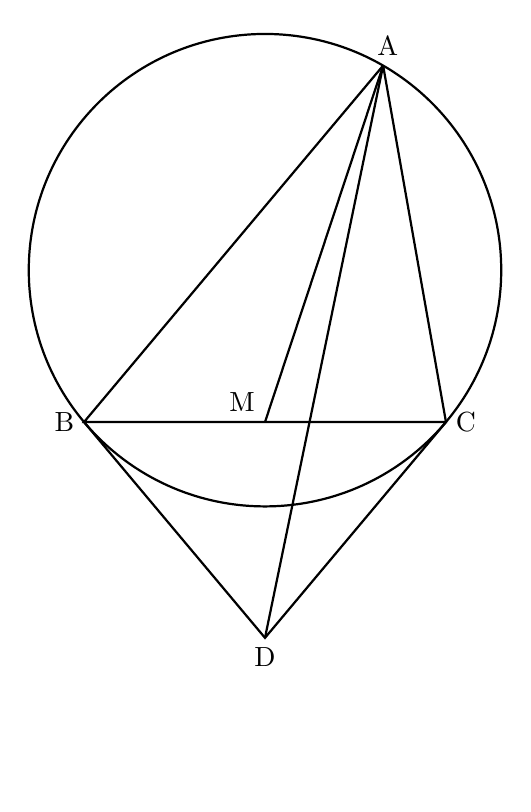
\begin{tikzpicture}[domain=-2.6:2.6,samples=70,scale=1.5]

		\coordinate (A) at (60:2) ;
		\coordinate (B) at (220:2) ; 
		\coordinate (C) at (320:2) ;
		\coordinate (O) at (0,0);
		
		\coordinate (X) at ($(B)!2!270:(O)$);
		\coordinate (Y) at ($(C)!2!90:(O)$);
		
		\coordinate (M) at ($(B)!0.5!(C)$);
		
		
		
		\draw [name path = Circle, thick] (0,0) circle (2);
		
		\draw (A) node [above] {\ A} ;
		\draw (B) node [left] {B} ;
		\draw (C) node [right] {C} ;
		%\draw (X) node [] {X} ;
		%\draw (Y) node [] {Y} ;
		
		\draw [thick] (A)--(B)--(C)--(A);
		
		\path [name path = BX] (B)--(X);
		\path [name path = CY] (C)--(Y);
		\path [name intersections={of=BX and CY,by={[label=below:D]D}}];
		
		\draw [thick] (B)--(D)--(C);
		\draw [thick] (A)--(M) node [above left] {M};
		\draw [thick] (A)--(D);
		
		%\node [draw] [thick] at (D) [circle through={(B)}] {};
\end{tikzpicture}


\bigskip


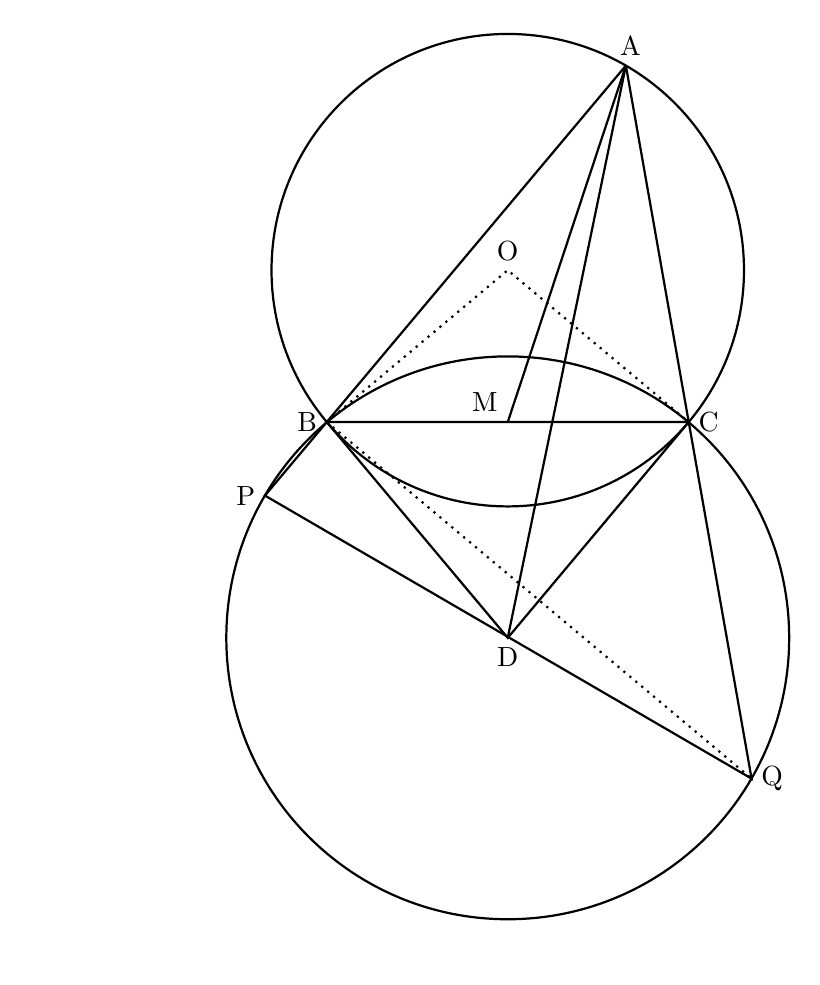
\begin{tikzpicture}[domain=-2.6:2.6,samples=70,scale=1.5]

		\coordinate (A) at (60:2) ;
		\coordinate (B) at (220:2) ; 
		\coordinate (C) at (320:2) ;
		\coordinate (O) at (0,0);
		
		\coordinate (X) at ($(B)!2!270:(O)$);
		\coordinate (Y) at ($(C)!2!90:(O)$);
		
		\coordinate (M) at ($(B)!0.5!(C)$);
		
		
		
		\draw [name path = Circle, thick] (0,0) circle (2);
		
		\draw (A) node [above] {\ A} ;
		\draw (B) node [left] {B} ;
		\draw (C) node [right] {C} ;
		\draw (O) node [above] {O} ;
		%\draw (X) node [] {X} ;
		%\draw (Y) node [] {Y} ;
		
		\draw [thick] (A)--(B)--(C)--(A);
		
		\path [name path = BX] (B)--(X);
		\path [name path = CY] (C)--(Y);
		\path [name intersections={of=BX and CY,by={[label=below:D]D}}];
		
		\draw [thick] (B)--(D)--(C);
		\draw [thick] (A)--(M) node [above left] {M};
		\draw [thick] (A)--(D);
		
		\node [draw] [thick ,name path = Circle_D] at (D) [circle through={(B)}] {};
		
		
		\path [name path = AB] (A)--($(A)!2!(B)$);
		\path [name path = AC] (A)--($(A)!2.5!(C)$);

		\path [name intersections={of=Circle_D and AB,by={,[label=left:P]P}}];
		\path [name intersections={of=Circle_D and AC,by={,[label=right:Q]Q}}];
		
		\draw [thick] (B)--(P)--(Q)--(C);
		
		\draw [thick, dotted] (B)--(O)--(C);
		\draw [thick, dotted] (B)--(Q);
		
\end{tikzpicture}






\newpage


\begin{tikzpicture}[domain=-2.6:2.6,samples=70,scale=1.5]

		\coordinate (B) at (153:2) ;
		\coordinate (C) at (27:2) ; 
		\coordinate (P) at (72:2) ;
		\coordinate (O) at (0,0);
		
		\coordinate (X) at ($(B)!2!90:(O)$);
		\coordinate (Y) at ($(C)!2!270:(O)$);
		
		\coordinate (M) at ($(B)!0.5!(C)$);
		
		%\draw [name path = Circle, thick] (0,0) circle (2);
		\path [name path = Circle, thick] (0,0) circle (2);
		
		\path [name path = AB] (B)--(X);
		\path [name path = AC] (C)--(Y);
		\path [name intersections={of=AB and AC,by={[label=above:A]A}}];

		
		%\draw (A) node [above] {\ A} ;
		\draw (B) node [left] {B} ;
		\draw (C) node [right] {C} ;
		%\draw (O) node [above] {O} ;
		\draw (M) node [below] {M} ;
		\draw (P) node [right] {P} ;
		%\draw (X) node [] {X} ;
		%\draw (Y) node [] {Y} ;
		
		\draw [thick] (A)--(B)--(C)--(A);
		\draw [thick] (P)--(A);
		\draw [thick] (P)--(B);
		\draw [thick] (P)--(C);
		\draw [thick] (P)--(M);
		
		\draw pic [draw, angle radius=5mm,angle eccentricity=1,pic text=$$] {angle = P--B--A}; %角度
		\draw pic [draw, angle radius=6mm,angle eccentricity=1,pic text=$$] {angle = P--B--A}; %角度
		\draw pic [draw, angle radius=5mm,angle eccentricity=1,pic text=$$] {angle = P--C--B}; %角度
		\draw pic [draw, angle radius=6mm,angle eccentricity=1,pic text=$$] {angle = P--C--B}; %角度

\end{tikzpicture}


\bigskip


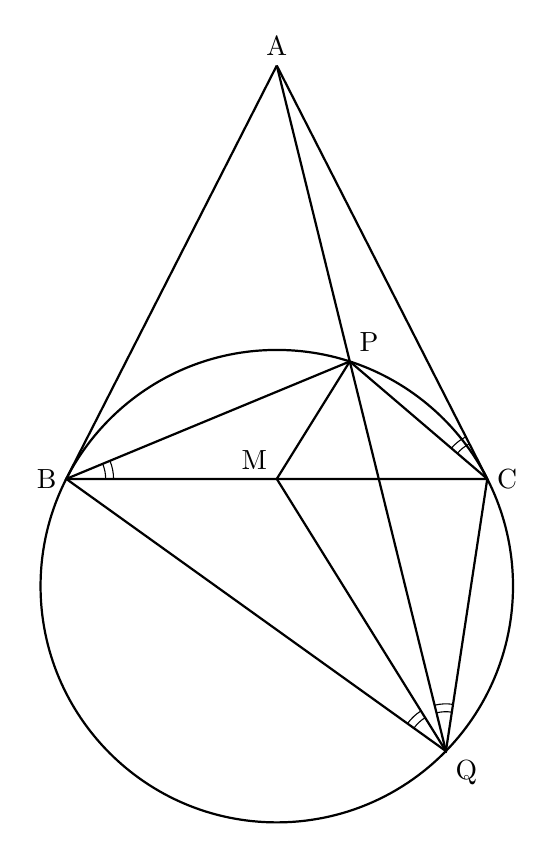
\begin{tikzpicture}[domain=-2.6:2.6,samples=70,scale=1.5]

		\coordinate (B) at (153:2) ;
		\coordinate (C) at (27:2) ; 
		\coordinate (P) at (72:2) ;
		\coordinate (O) at (0,0);
		
		\coordinate (X) at ($(B)!2!90:(O)$);
		\coordinate (Y) at ($(C)!2!270:(O)$);
		
		\coordinate (M) at ($(B)!0.5!(C)$);
		
		\draw [name path = Circle, thick] (0,0) circle (2);
		%\path [name path = Circle, thick] (0,0) circle (2);
		
		\path [name path = AB] (B)--(X);
		\path [name path = AC] (C)--(Y);
		\path [name intersections={of=AB and AC,by={[label=above:A]A}}];

		
		%\draw (A) node [above] {\ A} ;
		\draw (B) node [left] {B} ;
		\draw (C) node [right] {C} ;
		%\draw (O) node [above] {O} ;
		\draw (M) node [above left] {M} ;
		\draw (P) node [above right] {P} ;
		%\draw (X) node [] {X} ;
		%\draw (Y) node [] {Y} ;
		
		\draw [thick] (A)--(B)--(C)--(A);
		\draw [thick] (P)--(A);
		\draw [thick] (P)--(B);
		\draw [thick] (P)--(C);
		\draw [thick] (P)--(M);
		
		\draw pic [draw, angle radius=5mm,angle eccentricity=1,pic text=$$] {angle = C--B--P}; %角度
		\draw pic [draw, angle radius=6mm,angle eccentricity=1,pic text=$$] {angle = C--B--P}; %角度
		\draw pic [draw, angle radius=5mm,angle eccentricity=1,pic text=$$] {angle = A--C--P}; %角度
		\draw pic [draw, angle radius=6mm,angle eccentricity=1,pic text=$$] {angle = A--C--P}; %角度
		
		
		\path [name path = AP, thick] (A)--($(A)!2.5!(P)$);
		
		\path [name intersections={of=Circle and AP,by={, [label=below right:Q]Q}}];
		\draw [thick] (P)--(Q);
		\draw [thick] (B)--(Q)--(C);
		\draw [thick] (Q)--(M);
		
		\draw pic [draw, angle radius=5mm,angle eccentricity=1,pic text=$$] {angle = C--Q--A}; %角度
		\draw pic [draw, angle radius=6mm,angle eccentricity=1,pic text=$$] {angle = C--Q--A}; %角度
		\draw pic [draw, angle radius=5mm,angle eccentricity=1,pic text=$$] {angle = M--Q--B}; %角度
		\draw pic [draw, angle radius=6mm,angle eccentricity=1,pic text=$$] {angle = M--Q--B}; %角度
		
		
\end{tikzpicture}


\newpage 



\begin{tikzpicture}[domain=-2.6:2.6,samples=70,scale=1.2]

		\coordinate (A) at (270:2) ;
		\coordinate (P) at (160:2) ; 
		\coordinate (Q) at (60:2) ;
		\coordinate (O) at (0,0);
		
		
		\coordinate (M) at ($(B)!0.5!(C)$);
		
		\draw [name path = CircleG, thick] (0,0) circle (2);
		
		
		\draw (A) node [below] {A};
		\draw (P) node [above left] {P};
		\draw (Q) node [above] {Q};
		
		\path [name path = SP] (P)--($(P)!2!90:(O)$);
		\path [name path = SQ] (Q)--($(Q)!2!270:(O)$);
		\path [name intersections={of=SP and SQ,by={[label=above:S]S}}];
		
		\draw [name path = l,thick] ($(P)!1.8!(Q)$) node [right] {$l$}-- ($(Q)!1.8!(P)$);
		\draw [thick] (P)--(S)--(Q);
		
		
		
		\path [name path = Pver] (P)--($(P)!2!270:(Q)$);
		\coordinate (N) at ($(P)!0.5!(A)$);
		\path [name path = PAver] ($(N)!2!90:(P)$)--(N);
		\path [name intersections={of=Pver and PAver,by={[label=above:]O1}}];
		\node [draw] [thick ,name path = Circle_1] at (O1) [circle through={(P)}] {};


		\path [name path = Qver] (Q)--($(Q)!2!90:(P)$);
		\coordinate (L) at ($(Q)!0.5!(A)$);
		\path [name path = QAver] ($(L)!2!270:(Q)$)--(L);
		\path [name intersections={of=Qver and QAver,by={[label=above:]O2}}];
		\node [draw] [thick ,name path = Circle_2] at (O2) [circle through={(Q)}] {};
		
		
		\path [name intersections={of=Circle_1 and Circle_2 ,by={[label=above:B]B}}];
		
		
		\coordinate (H) at ($(P)!(B)!(Q)$);
		\coordinate (B') at ($(B)!2!(H)$);
		
		%\draw (B') node [] {B$'$};

		
\end{tikzpicture}



\begin{tikzpicture}[domain=-2.6:2.6,samples=70,scale=1.2]

		\coordinate (A) at (270:2) ;
		\coordinate (P) at (160:2) ; 
		\coordinate (Q) at (60:2) ;
		\coordinate (O) at (0,0);
		
		
		\coordinate (M) at ($(B)!0.5!(C)$);
		
		\draw [name path = CircleG, thick] (0,0) circle (2);
		
		
		\draw (A) node [below] {A};
		\draw (P) node [above left] {P};
		\draw (Q) node [above] {Q};
		
		\path [name path = SP] (P)--($(P)!2!90:(O)$);
		\path [name path = SQ] (Q)--($(Q)!2!270:(O)$);
		\path [name intersections={of=SP and SQ,by={[label=above:S]S}}];
		
		\draw [name path = l,thick] ($(P)!1.8!(Q)$) node [right] {$l$}-- ($(Q)!1.8!(P)$);
		\draw [thick] (P)--(S)--(Q);
		
		
		
		\path [name path = Pver] (P)--($(P)!2!270:(Q)$);
		\coordinate (N) at ($(P)!0.5!(A)$);
		\path [name path = PAver] ($(N)!2!90:(P)$)--(N);
		\path [name intersections={of=Pver and PAver,by={[label=above:]O1}}];
		\node [draw] [thick ,name path = Circle_1] at (O1) [circle through={(P)}] {};


		\path [name path = Qver] (Q)--($(Q)!2!90:(P)$);
		\coordinate (L) at ($(Q)!0.5!(A)$);
		\path [name path = QAver] ($(L)!2!270:(Q)$)--(L);
		\path [name intersections={of=Qver and QAver,by={[label=above:]O2}}];
		\node [draw] [thick ,name path = Circle_2] at (O2) [circle through={(Q)}] {};
		
		
		\path [name intersections={of=Circle_1 and Circle_2 ,by={[label=above:B]B}}];
		
		
		\coordinate (H) at ($(P)!(B)!(Q)$);
		\coordinate (B') at ($(B)!2!(H)$);
		
		%\draw (B') node [] {B$'$};

\end{tikzpicture}



\bigskip

\begin{tikzpicture}[domain=-2.6:2.6,samples=70,scale=1.2]

		\coordinate (A) at (270:2) ;
		\coordinate (P) at (160:2) ; 
		\coordinate (Q) at (60:2) ;
		\coordinate (O) at (0,0);
		
		
		\coordinate (M) at ($(B)!0.5!(C)$);
		
		\draw [name path = CircleG, thick] (0,0) circle (2);
		
		
		\draw (A) node [below] {A};
		\draw (P) node [above left] {P};
		\draw (Q) node [above] {Q};
		
		\path [name path = SP] (P)--($(P)!2!90:(O)$);
		\path [name path = SQ] (Q)--($(Q)!2!270:(O)$);
		\path [name intersections={of=SP and SQ,by={[label=above:S]S}}];
		
		\draw [name path = l,thick] ($(P)!1.8!(Q)$) node [right] {$l$}-- ($(Q)!1.8!(P)$);
		\draw [thick] (P)--(S)--(Q);
		
		
		
		\path [name path = Pver] (P)--($(P)!2!270:(Q)$);
		\coordinate (N) at ($(P)!0.5!(A)$);
		\path [name path = PAver] ($(N)!2!90:(P)$)--(N);
		\path [name intersections={of=Pver and PAver,by={[label=above:]O1}}];
		\node [draw] [thick ,name path = Circle_1, opacity=0.0] at (O1) [circle through={(P)}] {};


		\path [name path = Qver] (Q)--($(Q)!2!90:(P)$);
		\coordinate (L) at ($(Q)!0.5!(A)$);
		\path [name path = QAver] ($(L)!2!270:(Q)$)--(L);
		\path [name intersections={of=Qver and QAver,by={[label=above:]O2}}];
		\node [draw] [thick ,name path = Circle_2, opacity=0.0] at (O2) [circle through={(Q)}] {};
		
		
		\path [name intersections={of=Circle_1 and Circle_2 ,by={[label=below right:B]B}}];
		
		
		\coordinate (H) at ($(P)!(B)!(Q)$);
		\coordinate (B') at ($(B)!2!(H)$);
		
		\draw (B') node [above left] {R};
		
		\draw [thick] (A)--(P);
		\draw [thick] (A)--(S);
		\draw [thick] (A)--(Q);
		
		\coordinate (M) at ($(P)!0.5!(Q)$);
		\draw [thick] (A)--(M) node [above] {M};
		
		\draw [thick] (P)--(B)--(Q);
		\draw [thick, dotted] (P)--(B')--(Q);
		

\end{tikzpicture}


\bigskip

\begin{tikzpicture}[domain=-2.6:2.6,samples=70,scale=1.2]

		\coordinate (A) at (270:2) ;
		\coordinate (P) at (160:2) ; 
		\coordinate (Q) at (60:2) ;
		\coordinate (O) at (0,0);
		
		
		\coordinate (M) at ($(B)!0.5!(C)$);
		
		\path [name path = CircleG, thick] (0,0) circle (2);
		
		
		\draw (A) node [below] {A};
		\draw (P) node [above left] {P};
		\draw (Q) node [above] {Q};
		
		%\path [name path = SP] (P)--($(P)!2!90:(O)$);
		%\path [name path = SQ] (Q)--($(Q)!2!270:(O)$);
		%\path [name intersections={of=SP and SQ,by={[label=above:S]S}}];
		
		\draw [name path = l,thick] ($(P)!1.8!(Q)$) node [right] {$l$}-- ($(Q)!1.8!(P)$);
		%\draw [thick] (P)--(S)--(Q);
		
		
		
		\path [name path = Pver] (P)--($(P)!2!270:(Q)$);
		\coordinate (N) at ($(P)!0.5!(A)$);
		\path [name path = PAver] ($(N)!2!90:(P)$)--(N);
		\path [name intersections={of=Pver and PAver,by={[label=above:]O1}}];
		\node [draw] [thick ,name path = Circle_1] at (O1) [circle through={(P)}] {};


		\path [name path = Qver] (Q)--($(Q)!2!90:(P)$);
		\coordinate (L) at ($(Q)!0.5!(A)$);
		\path [name path = QAver] ($(L)!2!270:(Q)$)--(L);
		\path [name intersections={of=Qver and QAver,by={[label=above:]O2}}];
		\node [draw] [thick ,name path = Circle_2] at (O2) [circle through={(Q)}] {};
		
		
		\path [name intersections={of=Circle_1 and Circle_2 ,by={[label=right:B]B}}];
		
		
		\coordinate (H) at ($(P)!(B)!(Q)$);
		\coordinate (B') at ($(B)!2!(H)$);
		
		%\draw (B') node [] {B$'$};
		
		\coordinate (M) at ($(P)!0.5!(Q)$);
		\draw [thick] (A)--(M) node [above] {M};
		
		\draw [thick] (P)--(B)--(Q);
		\draw [thick] (P)--(A)--(Q);

\end{tikzpicture}








\vspace{10zw}











\newpage

%%%%%%%%%%%%%%%%%%%%%%%%%%%%%%%%%%%%%%%%%%%%%%%%%%%%%%%%内積
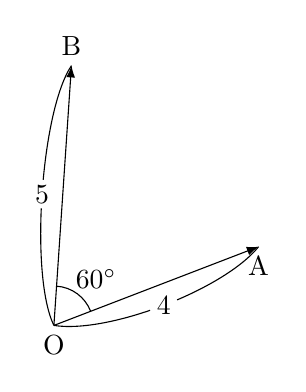
\begin{tikzpicture}[domain=-2.6:2.6,samples=70,scale=1]
    \usetikzlibrary{angles}
		
		\coordinate (a) at (0,0) node [below] {${\rm O}$};
		\coordinate (b) at (2.6,1) ; 
		\coordinate (c) at ($ (a)!.5!(b) $);
		\coordinate (d) at ($ (c)!3cm!90:(b) $);
		
		\draw (b)  node [below] {${\rm A}$};
		\draw (d)  node [above] {${\rm B}$};
		
		\draw [-{Latex[length=1.5mm]}] (a) -- (b) ;
		\draw [-{Latex[length=1.5mm]}] (a) -- (d) ;
				
		\draw pic [draw, angle radius=5mm,angle eccentricity=1,pic text=$$] {angle = b--a--d}; %角度
		\draw (48:8mm) node  {$60^{\circ}$}; %角度
		
		
		\draw [bend right,distance=0.7cm] (a)
         to node [fill=white,inner sep=0.8pt,circle] {4} (b); %長さ
         \draw [bend right,distance=0.7cm] (d)
         to node [fill=white,inner sep=0.8pt,circle] {5} (a); %長さ
         
%		\fill (d) circle (2.5pt) ;
\end{tikzpicture}


\begin{tikzpicture}[domain=-2.6:2.6,samples=70,scale=1]
    \usetikzlibrary{angles,calc}
		
		\coordinate (a) at (0,0) node [below] {${\rm O}$};
		\coordinate (b) at (4,0) ; 
		\coordinate (c) at ($ (a)!.5!(b) $);
		\coordinate (d) at ($ (c)!3cm!90:(b) $);
		
		\draw (b)  node [below] {${\rm A}$};
		\draw (d)  node [above] {${\rm B}$};
		
		\draw [-{Latex[length=1.5mm]}] (a) -- (b) ;
		\draw [-{Latex[length=1.5mm]}] (a) -- (d) ;
		
		\draw [dashed] (c) -- (d) ;
		
		 \draw [] ($(c)!8pt!(d)$)--($(c)!8pt!(d)!8pt!90:(c)$)--($(c)!8pt!(b)$); %角度
		
		\draw [bend right,distance=0.7cm] (a)
         to node [fill=white,inner sep=0.8pt,circle] {6} (b); %長さ
         \draw [bend right,distance=0.7cm] (c)
         to node [fill=white,inner sep=0.8pt,circle] {3} (a); %長さ
\end{tikzpicture}



\begin{tikzpicture}[domain=-2.6:2.6,samples=70,scale=1.2]
    \usetikzlibrary{angles}
		
\coordinate (a) at (0,0) node [below] {${\rm A}$};
		\coordinate (c) at (1,3) ; 
		\coordinate (b) at ($ (c)!1.7cm!90:(a)$);
		
		\draw (b)  node [right] {${\rm B}$};
		\draw (c)  node [above] {${\rm C}$};
		
		\draw [-] (a) -- (b) ;
		\draw [-] (a) -- (c) ;
		
		\draw [-] (c) -- (b) ;
		
		\draw [] ($(c)!8pt!(a)$)--($(c)!8pt!(a)!8pt!270:(c)$)--($(c)!8pt!(b)$); %角度
		
		\draw pic [draw, angle radius=5mm,angle eccentricity=1,pic text=$\hspace{-1zw}\theta$] {angle = c--b--a}; %角度
		%\draw (18:8mm) node  {$\theta$}; %角度
		
		
		\draw [bend right,distance=0.7cm] (a)
         to node [fill=white,inner sep=0.8pt,circle] {13} (b); %長さ
        \draw [bend right,distance=0.7cm] (c)
         to node [fill=white,inner sep=0.8pt,circle] {12} (a); %長さ
%		\fill (d) circle (2.5pt) ;
		
\end{tikzpicture}
    
    


\end{center}
\end{document}